\documentclass[border=4pt]{standalone}
\usepackage{tikz}
\usetikzlibrary{shapes.symbols,positioning,arrows.meta}

\begin{document}
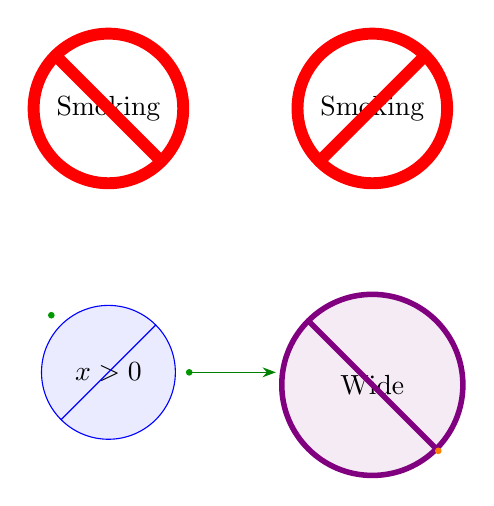
\begin{tikzpicture}[
  >=Stealth,
  node distance=13mm,
  sign/.style={draw=red,fill=white,line width=1ex,minimum size=19mm,align=center}
]
  \node[correct forbidden sign,sign] (correct) {Smoking};
  \node[forbidden sign,sign,right=of correct] (forbidden) {Smoking};
  \node[shape=forbidden sign,draw=blue,fill=blue!8,->,
    outer xsep=2pt,outer ysep=5pt,
    minimum size=17mm,below=of correct] (explicit) {$x>0$};
  \fill[green!60!black] (explicit.north west) circle (1.2pt);
  \fill[green!60!black] (explicit.east) circle (1.2pt);
  \draw[->,green!50!black] (explicit.east) -- ++(11mm,0) node[right] {east};
  \node[correct forbidden sign,draw=violet,fill=violet!8,line width=2pt,
    minimum width=23mm,minimum height=14mm,below=of forbidden] (wide) {Wide};
  \fill[orange] (wide.south east) circle (1.2pt);
\end{tikzpicture}
\end{document}
